% !TEX root = /media/ueslei/Ueslei/INPE/PCI/Projetos/Guia_COAWST/main.tex
\newpage
\thispagestyle{empty}

\begin{figure}[H]
    \centering
    \vspace*{\fill}
    
\includegraphics[width=0.35\textwidth]{loa_en.png}
    \vspace{0.5cm}
\end{figure}

\noindent\textsc{Ueslei Adriano Sutil} 
\\
 \textcolor{bleu_cite}{\href{mailto:uesleisutil1@gmail.com}{\textit{uesleisutil1@gmail.com}}}
\\  % URL
 \textcolor{bleu_cite}{\href{https://www.uesleisutil.com.br}{\textit{https://www.uesleisutil.com.br}}}
\bigskip

\noindent\textsc{Luciano Ponzi Pezzi}
\\
 \textcolor{bleu_cite}{\href{mailto:luciano.pezzi@inpe.br}{\textit{luciano.pezzi@inpe.br}}}  % URL
\bigskip
\\

 This guide is a contribution from the Ocean and Atmosphere Studies Laboratory (LOA)
to the scientific community. It was funded by the Institutional Training Scholarship from the National Institute for Space Research, 
through the Ministry of Science, Technology and Innovation and the National Council for Scientific and Technological Development (MCTI/CNPq) 
\textbf{process 301110/2017}.
\bigskip

 The image on the cover was taken by the first author during his second cruise to Antarctica,
in October 2017. It is licensed under a \textit{Creative Commons Attribution-NonCommercial-ShareAlike 4.0 International License}. 
\bigskip

 The image on the header of each chapter was taken by the first author during his first cruise to Antarctica, at Brazilian Antarctic Station Commander Ferraz, in October 2016. 
It is licensed under a \textit{Creative Commons Attribution-NonCommercial-ShareAlike 4.0 International License}. 
\bigskip

 The template \textit{Legrand Orange Book} was produced by Mathias Legrand (\textcolor{bleu_cite}{\href{mailto:legrand.mathias@gmail.com}{\textit{legrand.mathias@gmail.com}}}) 
and modified by Vel (\textcolor{bleu_cite}{\href{mailto:vel@latextemplates.com}{\textit{vel@latextemplates.com}}}) and Andrea Hidalgo (\textcolor{bleu_cite}{\href{mailto:andrea@inaoep.mx}{\textit{andrea@inaoep.mx}}}). 
It is licensed under a \textit{Creative Commons Attribution-NonCommercial 3.0 Unported}.
\bigskip

 The \textit{model2roms} toolbox (\textit{\textcolor{bleu_cite}{\href{https://github.com/trondkr/model2roms}{https://github.com/trondkr/model2roms}}}) was created by Trond 
          Kristiansen (\textit{\textcolor{bleu_cite}{\href{mailto:me@trondkristiansen.com}{me@trondkristiansen.com}}}) and is licensed under a \textit{MIT License}. 
\bigskip
\\

\noindent \href{http://creativecommons.org/licenses/by-nc-sa/4.0/}{
\includegraphics[width=0.1\textwidth]{cc.png}}% [1]
\\
 This work is licensed under a \textit{\textcolor{bleu_cite}{\href{http://creativecommons.org/licenses/by-nc-sa/4.0/}{Creative Commons Attribution-NonCommercial-ShareAlike 4.0 International License}}}.

\bigskip
\begin{flushleft}
 \textbf{Third edition} 
\\ 
 \textbf{November 2020} 
\\
\end{flushleft}

\begin{figure}[H]
    \centering
    \vspace*{\fill}
    
\includegraphics[width=0.25\textwidth]{cnpq.png}
    \hspace{3cm}
    
\includegraphics[width=0.12\textwidth]{capes.jpg}
    \hspace{3cm}    
    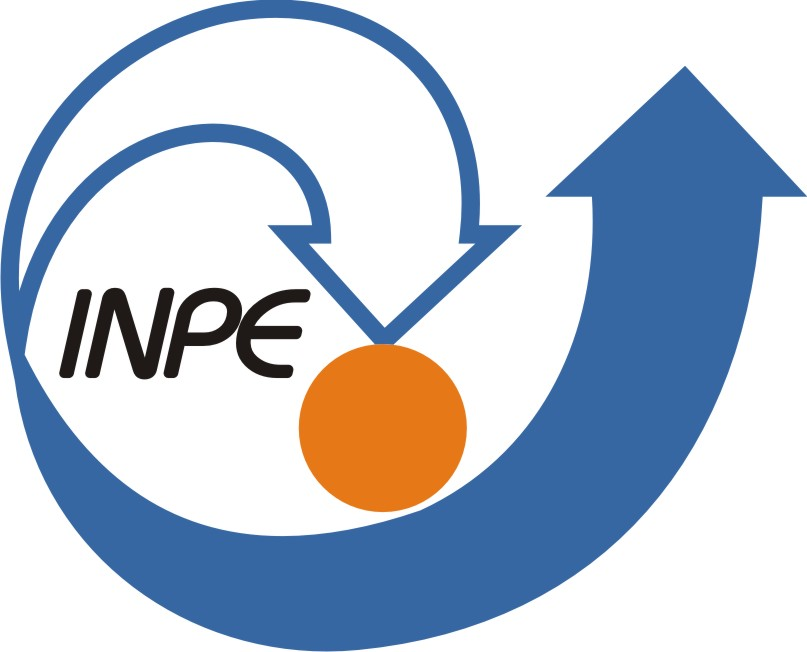
\includegraphics[width=0.13\textwidth]{inpe.jpg}
\end{figure}
